\section{Testing the Software}

\subsection{Rendering (\ref{req_rendering})}

\subsubsection{High-Quality Rendering (1.1, 1.2, 1.3 and 1.4)}

These requirements revolve around correctly and accurately rendering fractals, which the images below demonstrate. The left image shows the Mandelbrot set, with the right image (a zoomed-in portion of the former) showing no artefacts in the render. Both images are pleasantly coloured, and the fractal details are clearly highlighted.

\FloatBarrier
\begin{figure*}[htp]
	\centering
	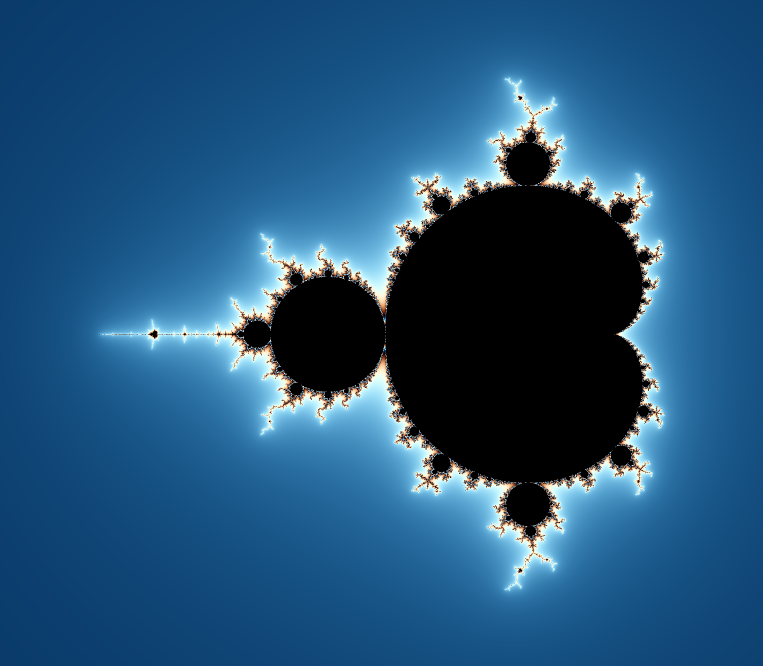
\includegraphics[width=.435\textwidth]{requirement1.1.png}
	
\includegraphics[width=.4\textwidth]{requirement1.1_2.png}
\end{figure*}
\FloatBarrier

\subsubsection{Anti-Aliasing (1.5)}

Anti-aliasing the render makes it appear much smoother and reduces pixelation in the image. The two images below show the difference between rendering the image with and without anti-aliasing (they are rendered at a low resolution to emphasise the differences). The image on the right is rendered with anti-aliasing, while the image on the left is not.

\FloatBarrier
\begin{figure*}[htp]
	\centering
	
\includegraphics[width=.4175\textwidth]{requirement1.5.png}
	
\includegraphics[width=.4175\textwidth]{requirement1.5_2.png}
\end{figure*}
\FloatBarrier

\subsubsection{Image Resizing (1.6)}

The images below show the same portion of the Mandelbrot set but rendered at different resolutions. The lower the resolution, the quicker the image renders, but the worse it looks.

\FloatBarrier
\begin{figure*}[htp]
	\centering
	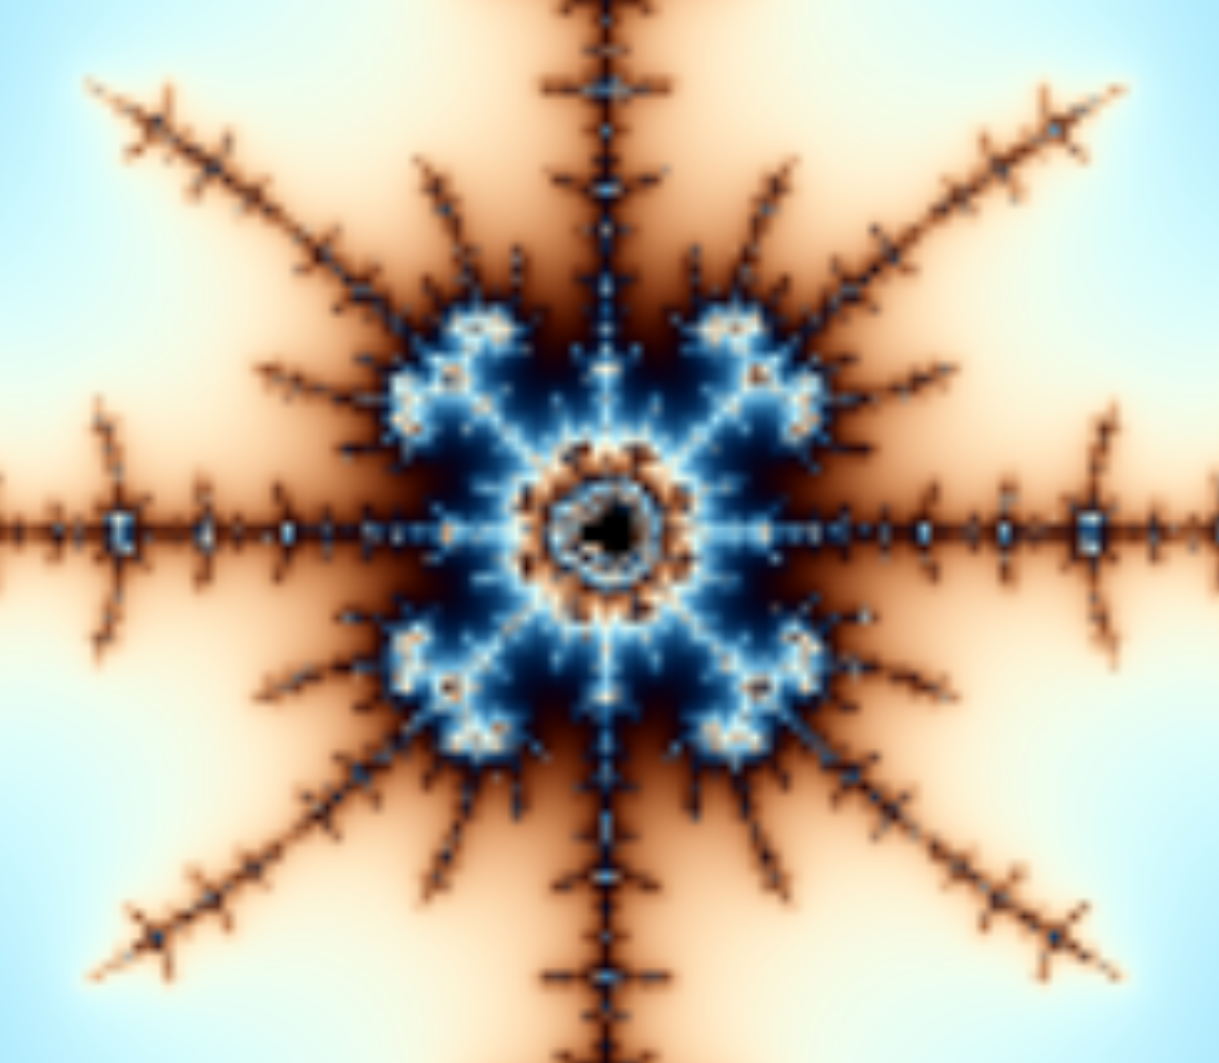
\includegraphics[width=.4175\textwidth]{requirement1.6.png}
	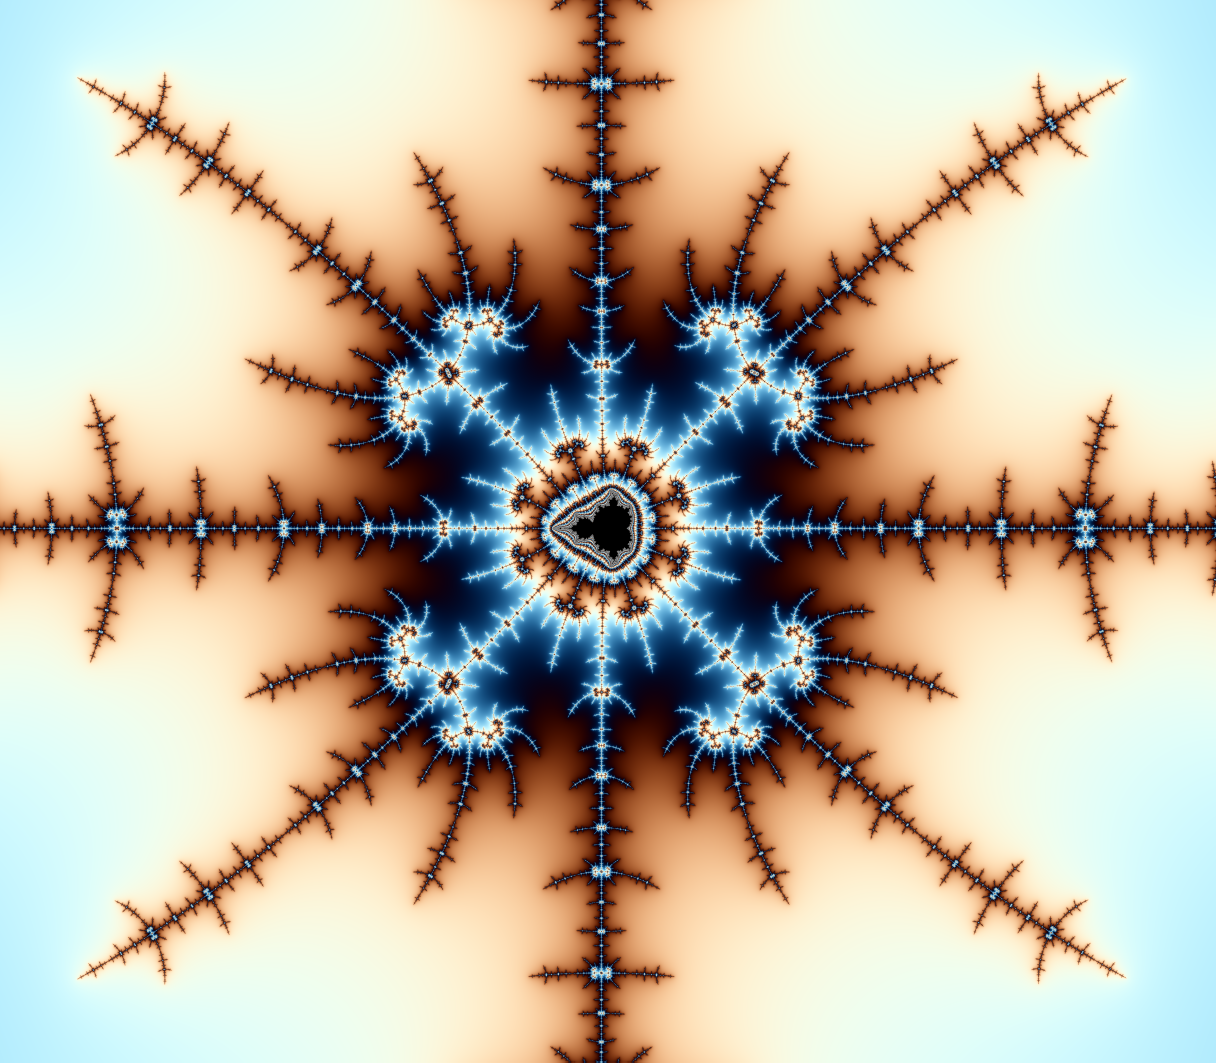
\includegraphics[width=.4175\textwidth]{requirement1.6_2.png}
\end{figure*}
\FloatBarrier

\subsubsection{Optimisations (1.7, 1.8)}

The only algorithmic optimisation that was practical to implement within this project's scope was the outline detection method of accelerating the rendering of some fractal regions. The image below shows, in red, the render boxes whose perimeters were entirely contained within the Mandelbrot set and hence contained only points in the set.

\FloatBarrier
\begin{figure*}[htp]
	\centering
	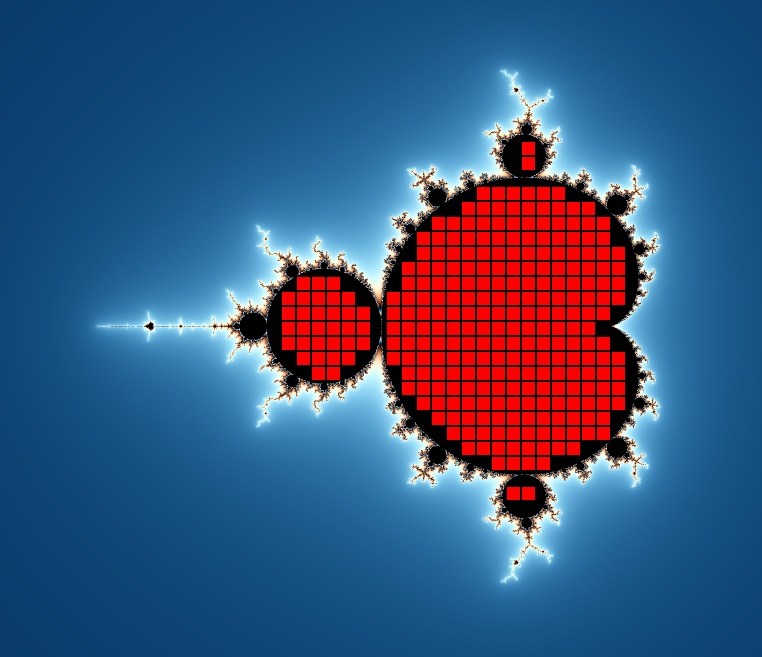
\includegraphics[width=.6\textwidth]{requirement1.8.png}
\end{figure*}
\FloatBarrier

\subsubsection{Infinite Zooming (1.9)}

When the user zooms into a factor of around $1 \times 10 ^{14}$, the precision of a 64-bit floating point value leads to significant rendering artefacts. To circumvent this, the program supports arbitrary-precision floating point types implemented in software. These make the rendering process much slower but allow for near-infinite zooming.

The image on the left shows the fractal rendered with 64-bit precision, while the image on the left shows the same point rendered with 128-bit precision.

\FloatBarrier
\begin{figure*}[htp]
	\centering
	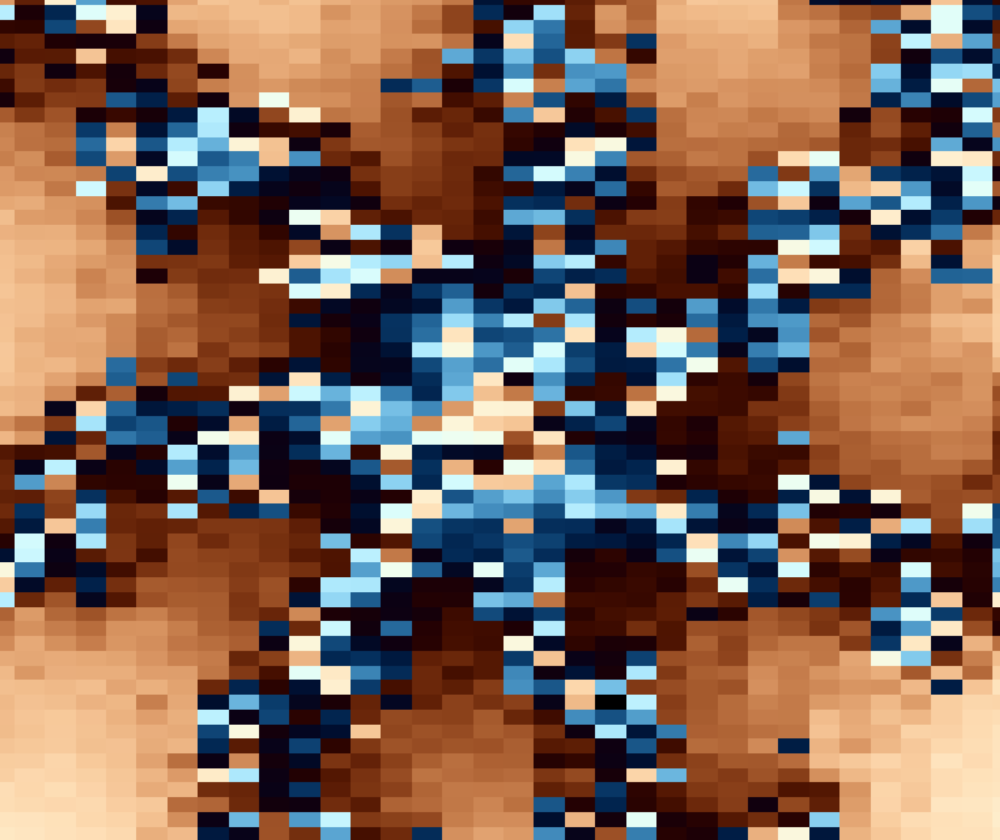
\includegraphics[width=.4175\textwidth]{requirement1.9.png}
	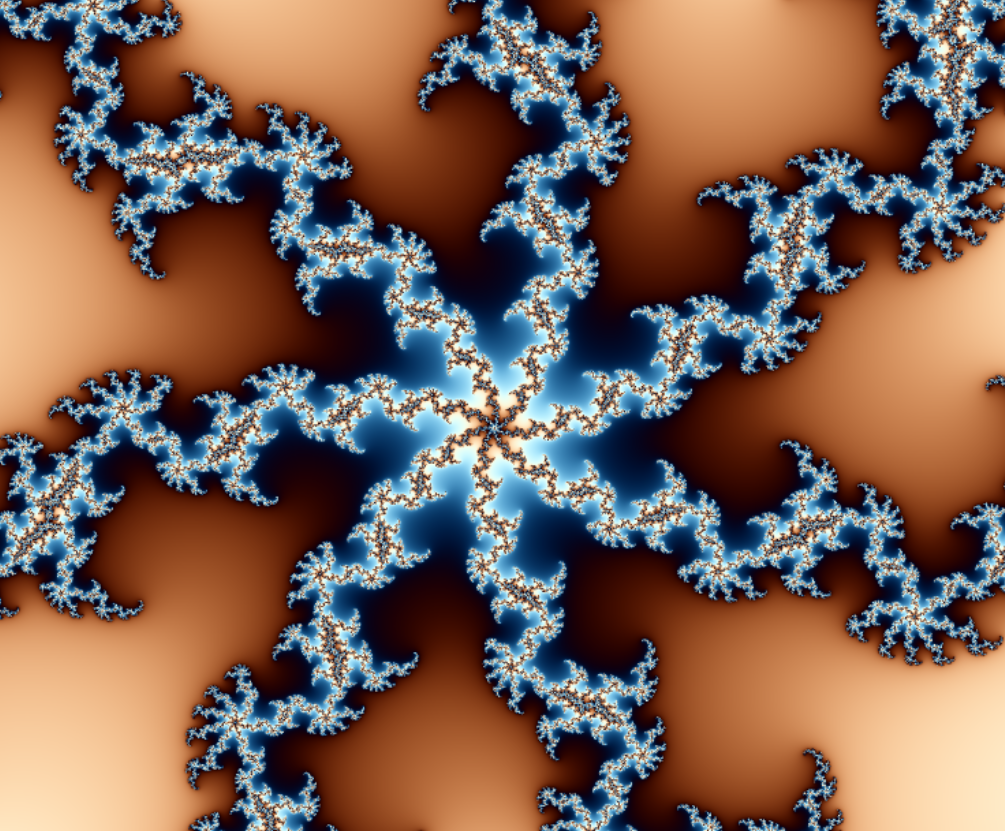
\includegraphics[width=.4175\textwidth]{requirement1.9_2.png}
\end{figure*}
\FloatBarrier


\subsection{Configuration (\ref{req_configuration})}

\subsubsection{Zoom Factor and Fractal Position (2.1)}

The zoom factor and fractal position can be adjusted in two main ways. The first way is to change the \codeword{settings.json} file directly, entering custom coordinates and dimensions for the fractal. The second and much easier way is implemented and tested in various sections of requirement 3 (``Interface and Movement'').

\subsubsection{Fractal Render Configurations (2.2, 2.3, 2.4, 2.5)}

For the program to be fully customisable, the number of threads, anti-aliasing factor, etc., must be configurable. The window responsible for providing these options is shown below.

Note that while the bailout value cannot be changed directly from this menu (since it does not significantly change the appearance of the resulting image), it can be changed from within the \codeword{settings.json} file.

\FloatBarrier
\begin{figure*}[htp]
	\centering
	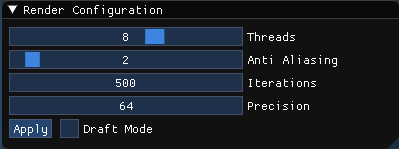
\includegraphics[width=.835\textwidth]{requirement2.2.png}
\end{figure*}
\FloatBarrier

\subsubsection{Image Resizing (2.6, 2.7)}

The ability to resize the image (both drawn size and rendered size) has been demonstrated in previous points (notably in 1.6)

\subsubsection{Colouring Algorithms (2.8)}

The colouring algorithm can be changed by selecting an option in a simple drop-down menu. The images below show three different colouring methods applied to the same fractal. The middle two algorithms support custom colour palettes, which can be defined in the \codeword{settings.json} file and loaded from another drop-down menu.

\FloatBarrier
\begin{figure*}[htp]
	\centering
	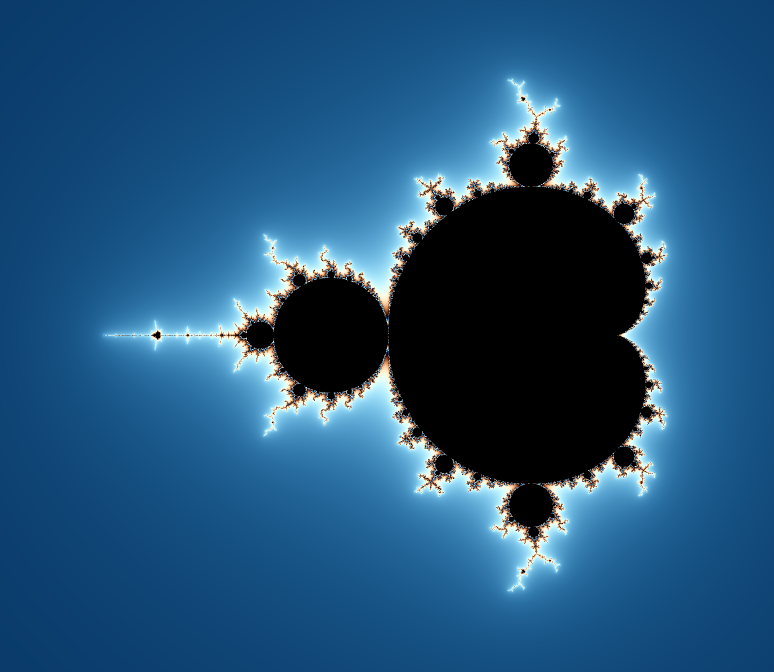
\includegraphics[width=.243\textwidth]{requirement2.8.png}
	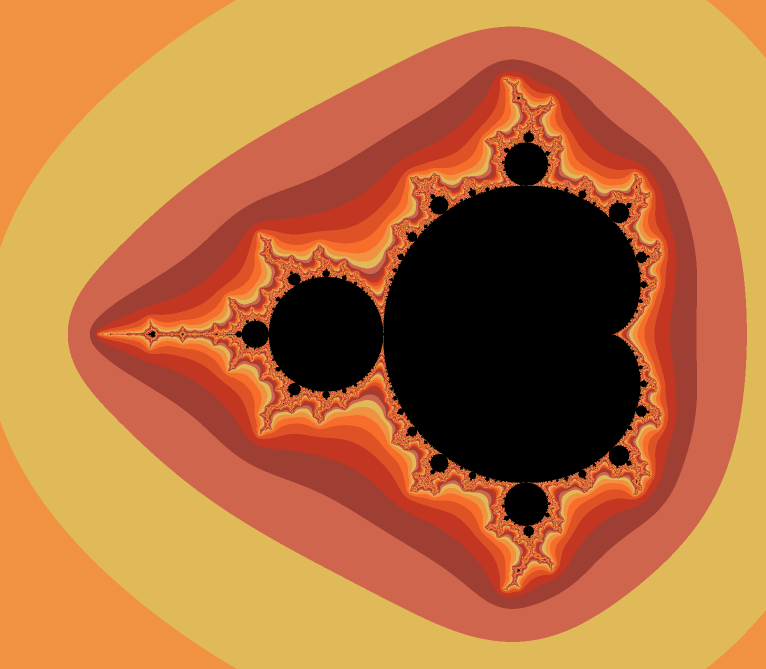
\includegraphics[width=.243\textwidth]{requirement2.8_2.png}
	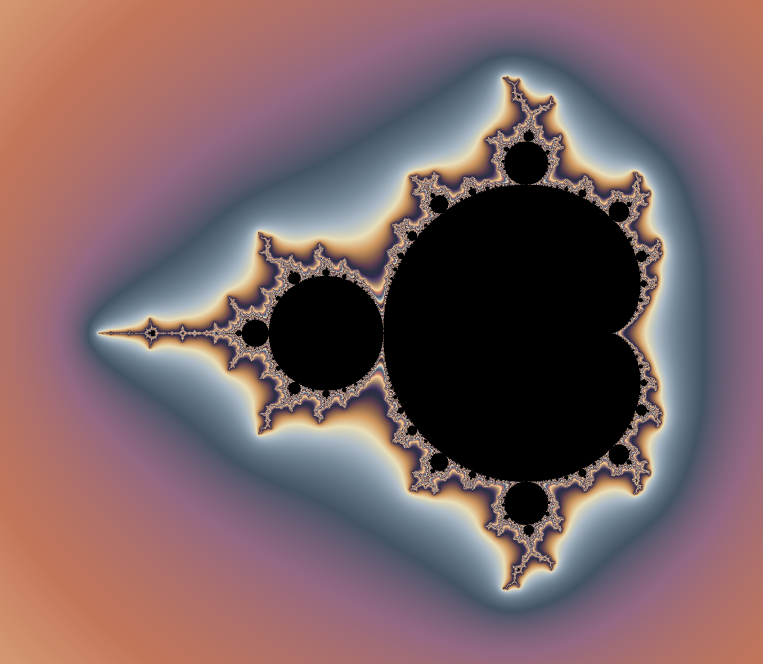
\includegraphics[width=.243\textwidth]{requirement2.8_3.png}
	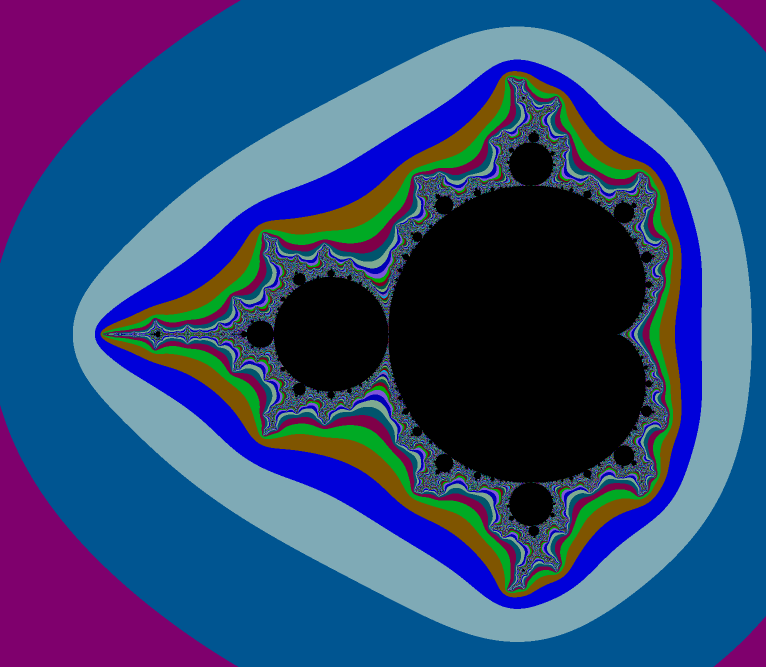
\includegraphics[width=.243\textwidth]{requirement2.8_4.png}
\end{figure*}
\FloatBarrier

\subsubsection{Default Settings (2.9)}

A single button in the \codeword{Fractal Settings} window enables the user to reset the fractal to its default configuration, which is defined by the \codeword{settings.json} file.

% Padding
\pagebreak
\subsubsection{History (2.10)}

\FloatBarrier
\begin{center}
	\begin{figure}[htbp]
		\begin{minipage}{0.8\linewidth}
			The software implements a fully-functional history, featuring undoing and redoing with keyboard controls and a visual representation of the history supporting mouse selection. The image to the right shows a small example of this.
		\end{minipage}
		\hfill
		\begin{minipage}{0.15\linewidth}
			\centering
			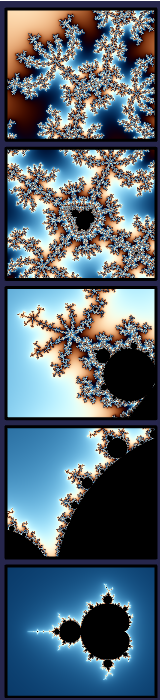
\includegraphics[width=\linewidth]{requirement2.10.png}
		\end{minipage}
	\end{figure}
\end{center}
\FloatBarrier

\subsubsection{Arbitrary Precision Arithmetic (2.11)}

The ability to change the precision of the floating point arithmetic performed has been demonstrated in 1.9, with the precision input box shown in 2.2 to 2.5.

\subsubsection{Support for More Fractals (2.12)}

The software implements the Mandelbrot Set, a variant of the Julia Set and Newton's Fractal. These fractals are shown below, in that order.

\FloatBarrier
\begin{figure*}[htp]
	\centering
	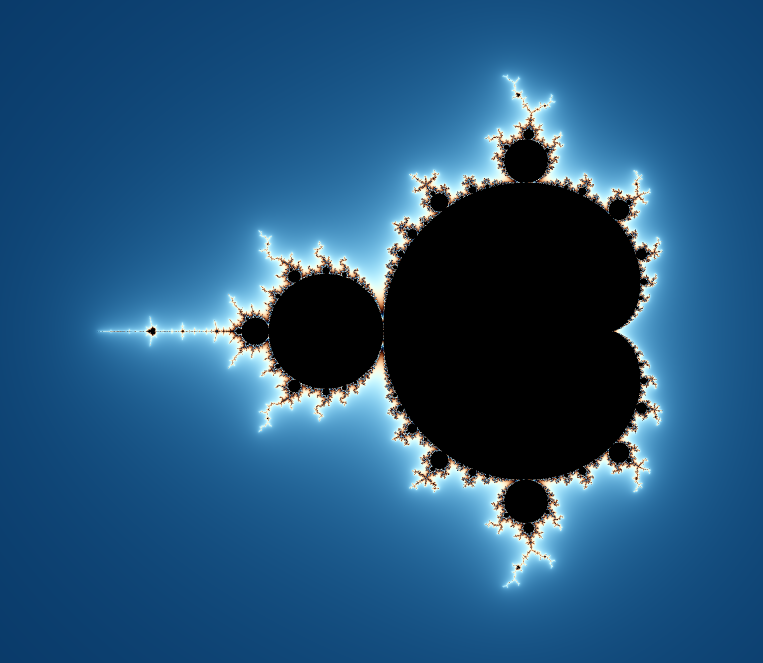
\includegraphics[width=.323\textwidth]{requirement2.12.png}
	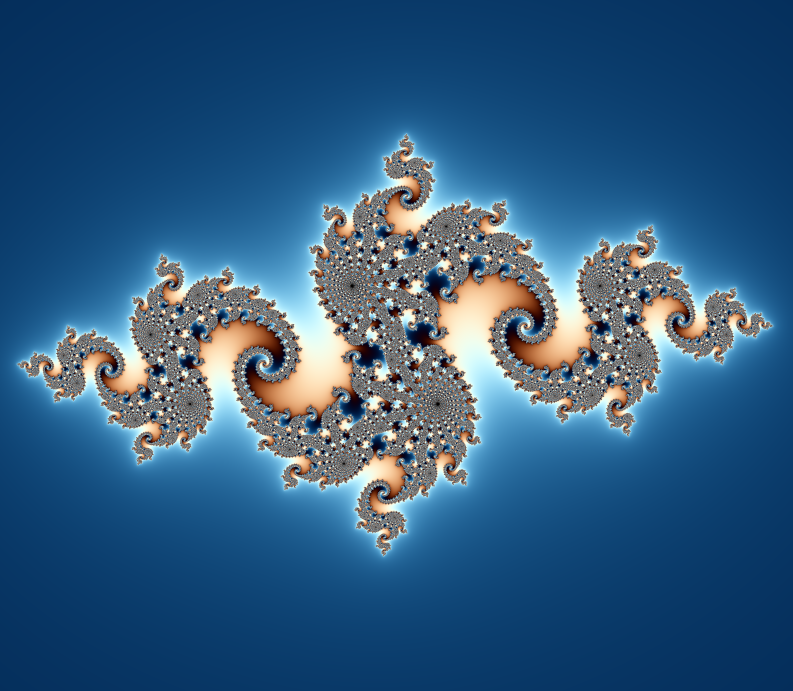
\includegraphics[width=.323\textwidth]{requirement2.12_2.png}
	
\includegraphics[width=.323\textwidth]{requirement2.12_3.png}
\end{figure*}
\FloatBarrier

\subsubsection{Default Settings on Changing Fractal (2.13)}

Having spent more time developing the software, I realised that implementing this as a feature may not be a good idea since the user could accidentally pick a different fractal and wish to return or want to see how different fractals behave at the same point. As a result, this feature will not be implemented, but the reset button described in 2.9 will allow the user to reset the fractal type.

\subsubsection{Settings as a JSON File (2.14)}

The entire render configuration is described in a single JSON file (\codeword{settings/settings.json}) loaded when the program first runs. By default, it renders the Mandelbrot set since it is the most well-known fractal by many.


\subsection{Interface and Movement (\ref{req_interface})}

\subsubsection{Graphical User Interface (3.1, 3.2, 3.3, 3.4)}

A range of GUI windows show all the information required for fine-grained fractal manipulation. What is shown in each window will change depending on the currently selected options, such as the precision, whether a draft render is being performed or whether a valid file path has been entered.

\FloatBarrier
\begin{figure*}[htp]
	\centering
	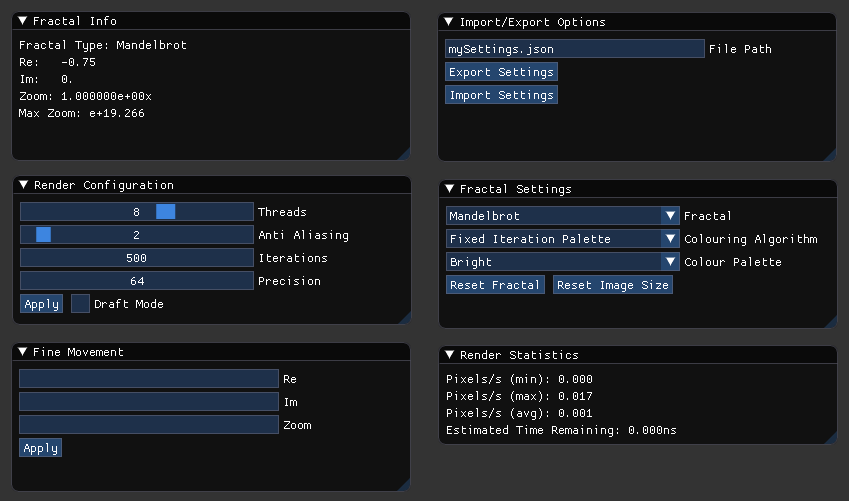
\includegraphics[width=\textwidth]{requirement3.1.png}
\end{figure*}
\FloatBarrier

\vspace{0.25cm}
The image below shows the \codeword{Fractal Info} window when using 128-bit precision zoomed in to a factor of $1 \times 10^{30}$. This shows the software can display text versions of high-precision floating point values within its windows.

\FloatBarrier
\begin{figure*}[htp]
	\centering
	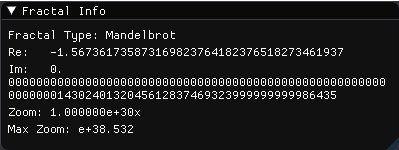
\includegraphics[width=0.6\textwidth]{requirement3.4.png}
\end{figure*}
\FloatBarrier

\subsubsection{Window Positioning (3.5, 3.6)}

While it may be useful for some of the more advanced menus to be hidden from complete beginners, the more advanced settings are contained in separate windows and can be easily ignored. Furthermore, given the simplicity of the settings configurations and the ease with which things can be changed and reset, it may even be beneficial for new users to experiment with unfamiliar settings.

\subsubsection{Zoom Box Selection (3.7, 3.8, 3.9)}

Zoom selection can be performed by dragging the mouse, which creates a red box indicating where the zoom will occur. Pressing enter will accept the zoom, and pressing escape or drawing a new box will cancel the existing one. The image below shows an example of this.

\FloatBarrier
\begin{figure*}[htp]
	\centering
	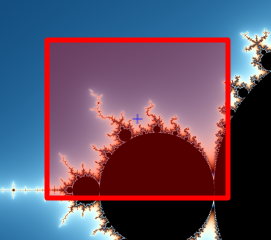
\includegraphics[width=0.4\textwidth]{requirement3.7.png}
\end{figure*}
\FloatBarrier

\vspace{0.5cm}

The zoom box could be drawn at any aspect ratio early in the development process. While this had some benefits, the cost was that the fractal would often end up being distorted and stretched, which was unattractive and difficult to fix. As a result, some functions were implemented to ensure that the box always remains aspect-corrected for the size of the fractal, meaning it can't become distorted.

Furthermore, the zoom box can be moved by clicking inside the box and dragging it around. This, combined with the small cross in the middle of the box, allows the user to zoom in on the desired location more precisely.

\subsubsection{Render Progress (3.10)}

The \codeword{Render Statistics} window shows the current progress of the fractal render and the estimated remaining time. The time is formatted and automatically adjusted to the most suitable units. For example, if there are 300 seconds left of the render, the time will be displayed as $5 \mathrm{m}$.

\FloatBarrier
\begin{figure*}[htp]
	\centering
	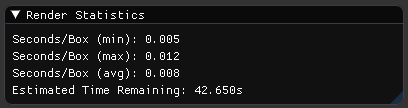
\includegraphics[width=0.5\textwidth]{requirement3.10.png}
\end{figure*}
\FloatBarrier

\subsubsection{Move History (3.11, 3.12)}

The history is described in more detail in 2.10 and can be used to zoom back out of the fractal. Furthermore, it is possible to reset the fractal, which has the effect of zooming out. An alternative solution is to change the zoom factor directly.

\subsubsection{Progressive Rendering (3.13)}

The software implements a ``draft mode'', which renders only a few pixels per box. Increasing the step reduces the number of pixels rendered, increasing speed but reducing the apparent quality of the render.

\FloatBarrier
\begin{figure*}[htp]
	\centering
	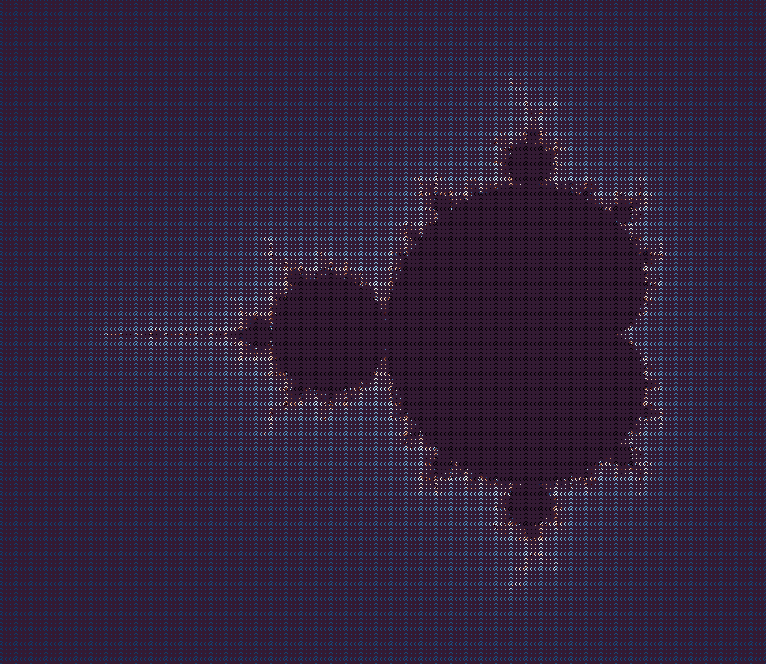
\includegraphics[width=0.6\textwidth]{requirement3.13.png}
\end{figure*}
\FloatBarrier

\subsubsection{Maximum Zoom (3.14)}

As shown in 3.1 to 3.4, the maximum zoom possible is shown in the window. This is calculated based on the current precision and is an absolute upper bound. It gives the user a rough estimate of how deep they can zoom before the fractal quality starts to deteriorate.

\subsubsection{Scientific Input (3.15)}

Using MPIR's string processing functionality, the numeric input fields can all accept scientific inputs.

\FloatBarrier
\begin{figure*}[htp]
	\centering
	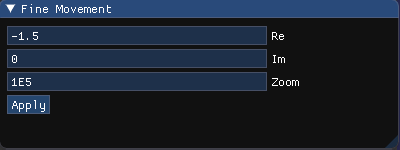
\includegraphics[width=0.6\textwidth]{requirement3.15.png}
\end{figure*}
\FloatBarrier

\subsection{Import and Export (\ref{req_import_export})}

\subsubsection{Import and Export of Settings (4.1, 4.2)}

The settings export option only appears when a valid file extension is supplied (JSON or text). When this is the case, the options to export or import the settings are shown. If there are any errors in the file opening or writing process, they are caught and handled gracefully.

\FloatBarrier
\begin{figure*}[htp]
	\centering
	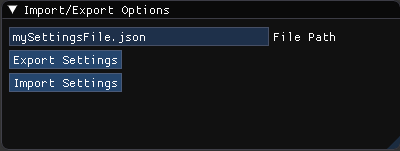
\includegraphics[width=0.6\textwidth]{requirement4.1.png}
\end{figure*}
\FloatBarrier

\subsubsection{Saving Images (4.3, 4.4, 4.5)}

Images can be saved in the same way as the settings configuration and with many common file extensions. Currently, it is not possible to render images separately from the main program, but this could be implemented by creating a new \codeword{FractalRenderer} instance, initializing it, triggering a render and saving it to a file.

\subsection{Installation (\ref{req_install})}

\subsubsection{Compilation and Platform Support (5.1, 5.2, 5.3, 5.4, 5.5, 5.6, 5.7)}

The software is easy to compile on Windows with CMake and MSVC, with the required steps shown below. Compiling on MacOS and Linux is untested, as I have no means of compiling the software on these platforms. The code should, however, compile and run correctly since all of the included libraries are known to work cross-platform.

\begin{lstlisting}[]
	git clone --recursive https://github.com/Pencilcaseman/FractalRenderer.git
	cd FractalRenderer
	mkdir build
	cd build
	cmake .. -DCMAKE_BUILD_TYPE=Release
	cmake --build . --config Release --parallel
\end{lstlisting}

\subsection{Performance (\ref{req_performance})}

As seen previously, the code is capable of rendering images at machine precision and above. The time taken for these renders depends heavily on the computer used, the fractal type, the area of the fractal being rendered and more. Luckily, the code is fast enough for all reasonable configurations with machine precision, and the renders finish very quickly (often in less than 50ms).

To increase the performance of the renderer, there are a few main options:

\begin{enumerate}
	\item Use a draft render
	\item Lower the quality of the render
	\item Lower the resolution of the render
	\item Use more threads
	\item Use machine word precision instead of arbitrary precision arithmetic
\end{enumerate}
